% Options for packages loaded elsewhere
\PassOptionsToPackage{unicode}{hyperref}
\PassOptionsToPackage{hyphens}{url}
\PassOptionsToPackage{dvipsnames,svgnames,x11names}{xcolor}
%
\documentclass[
  letterpaper,
  DIV=11,
  numbers=noendperiod]{scrartcl}

\usepackage{amsmath,amssymb}
\usepackage{iftex}
\ifPDFTeX
  \usepackage[T1]{fontenc}
  \usepackage[utf8]{inputenc}
  \usepackage{textcomp} % provide euro and other symbols
\else % if luatex or xetex
  \usepackage{unicode-math}
  \defaultfontfeatures{Scale=MatchLowercase}
  \defaultfontfeatures[\rmfamily]{Ligatures=TeX,Scale=1}
\fi
\usepackage{lmodern}
\ifPDFTeX\else  
    % xetex/luatex font selection
\fi
% Use upquote if available, for straight quotes in verbatim environments
\IfFileExists{upquote.sty}{\usepackage{upquote}}{}
\IfFileExists{microtype.sty}{% use microtype if available
  \usepackage[]{microtype}
  \UseMicrotypeSet[protrusion]{basicmath} % disable protrusion for tt fonts
}{}
\makeatletter
\@ifundefined{KOMAClassName}{% if non-KOMA class
  \IfFileExists{parskip.sty}{%
    \usepackage{parskip}
  }{% else
    \setlength{\parindent}{0pt}
    \setlength{\parskip}{6pt plus 2pt minus 1pt}}
}{% if KOMA class
  \KOMAoptions{parskip=half}}
\makeatother
\usepackage{xcolor}
\setlength{\emergencystretch}{3em} % prevent overfull lines
\setcounter{secnumdepth}{-\maxdimen} % remove section numbering
% Make \paragraph and \subparagraph free-standing
\makeatletter
\ifx\paragraph\undefined\else
  \let\oldparagraph\paragraph
  \renewcommand{\paragraph}{
    \@ifstar
      \xxxParagraphStar
      \xxxParagraphNoStar
  }
  \newcommand{\xxxParagraphStar}[1]{\oldparagraph*{#1}\mbox{}}
  \newcommand{\xxxParagraphNoStar}[1]{\oldparagraph{#1}\mbox{}}
\fi
\ifx\subparagraph\undefined\else
  \let\oldsubparagraph\subparagraph
  \renewcommand{\subparagraph}{
    \@ifstar
      \xxxSubParagraphStar
      \xxxSubParagraphNoStar
  }
  \newcommand{\xxxSubParagraphStar}[1]{\oldsubparagraph*{#1}\mbox{}}
  \newcommand{\xxxSubParagraphNoStar}[1]{\oldsubparagraph{#1}\mbox{}}
\fi
\makeatother


\providecommand{\tightlist}{%
  \setlength{\itemsep}{0pt}\setlength{\parskip}{0pt}}\usepackage{longtable,booktabs,array}
\usepackage{calc} % for calculating minipage widths
% Correct order of tables after \paragraph or \subparagraph
\usepackage{etoolbox}
\makeatletter
\patchcmd\longtable{\par}{\if@noskipsec\mbox{}\fi\par}{}{}
\makeatother
% Allow footnotes in longtable head/foot
\IfFileExists{footnotehyper.sty}{\usepackage{footnotehyper}}{\usepackage{footnote}}
\makesavenoteenv{longtable}
\usepackage{graphicx}
\makeatletter
\def\maxwidth{\ifdim\Gin@nat@width>\linewidth\linewidth\else\Gin@nat@width\fi}
\def\maxheight{\ifdim\Gin@nat@height>\textheight\textheight\else\Gin@nat@height\fi}
\makeatother
% Scale images if necessary, so that they will not overflow the page
% margins by default, and it is still possible to overwrite the defaults
% using explicit options in \includegraphics[width, height, ...]{}
\setkeys{Gin}{width=\maxwidth,height=\maxheight,keepaspectratio}
% Set default figure placement to htbp
\makeatletter
\def\fps@figure{htbp}
\makeatother
% definitions for citeproc citations
\NewDocumentCommand\citeproctext{}{}
\NewDocumentCommand\citeproc{mm}{%
  \begingroup\def\citeproctext{#2}\cite{#1}\endgroup}
\makeatletter
 % allow citations to break across lines
 \let\@cite@ofmt\@firstofone
 % avoid brackets around text for \cite:
 \def\@biblabel#1{}
 \def\@cite#1#2{{#1\if@tempswa , #2\fi}}
\makeatother
\newlength{\cslhangindent}
\setlength{\cslhangindent}{1.5em}
\newlength{\csllabelwidth}
\setlength{\csllabelwidth}{3em}
\newenvironment{CSLReferences}[2] % #1 hanging-indent, #2 entry-spacing
 {\begin{list}{}{%
  \setlength{\itemindent}{0pt}
  \setlength{\leftmargin}{0pt}
  \setlength{\parsep}{0pt}
  % turn on hanging indent if param 1 is 1
  \ifodd #1
   \setlength{\leftmargin}{\cslhangindent}
   \setlength{\itemindent}{-1\cslhangindent}
  \fi
  % set entry spacing
  \setlength{\itemsep}{#2\baselineskip}}}
 {\end{list}}
\usepackage{calc}
\newcommand{\CSLBlock}[1]{\hfill\break\parbox[t]{\linewidth}{\strut\ignorespaces#1\strut}}
\newcommand{\CSLLeftMargin}[1]{\parbox[t]{\csllabelwidth}{\strut#1\strut}}
\newcommand{\CSLRightInline}[1]{\parbox[t]{\linewidth - \csllabelwidth}{\strut#1\strut}}
\newcommand{\CSLIndent}[1]{\hspace{\cslhangindent}#1}

\usepackage{booktabs}
\usepackage{longtable}
\usepackage{array}
\usepackage{multirow}
\usepackage{wrapfig}
\usepackage{float}
\usepackage{colortbl}
\usepackage{pdflscape}
\usepackage{tabu}
\usepackage{threeparttable}
\usepackage{threeparttablex}
\usepackage[normalem]{ulem}
\usepackage{makecell}
\usepackage{xcolor}
\usepackage{float}
\usepackage{placeins}
\KOMAoption{captions}{tableheading}
\makeatletter
\@ifpackageloaded{caption}{}{\usepackage{caption}}
\AtBeginDocument{%
\ifdefined\contentsname
  \renewcommand*\contentsname{Table of contents}
\else
  \newcommand\contentsname{Table of contents}
\fi
\ifdefined\listfigurename
  \renewcommand*\listfigurename{List of Figures}
\else
  \newcommand\listfigurename{List of Figures}
\fi
\ifdefined\listtablename
  \renewcommand*\listtablename{List of Tables}
\else
  \newcommand\listtablename{List of Tables}
\fi
\ifdefined\figurename
  \renewcommand*\figurename{Figure}
\else
  \newcommand\figurename{Figure}
\fi
\ifdefined\tablename
  \renewcommand*\tablename{Table}
\else
  \newcommand\tablename{Table}
\fi
}
\@ifpackageloaded{float}{}{\usepackage{float}}
\floatstyle{ruled}
\@ifundefined{c@chapter}{\newfloat{codelisting}{h}{lop}}{\newfloat{codelisting}{h}{lop}[chapter]}
\floatname{codelisting}{Listing}
\newcommand*\listoflistings{\listof{codelisting}{List of Listings}}
\makeatother
\makeatletter
\makeatother
\makeatletter
\@ifpackageloaded{caption}{}{\usepackage{caption}}
\@ifpackageloaded{subcaption}{}{\usepackage{subcaption}}
\makeatother

\ifLuaTeX
  \usepackage{selnolig}  % disable illegal ligatures
\fi
\usepackage{bookmark}

\IfFileExists{xurl.sty}{\usepackage{xurl}}{} % add URL line breaks if available
\urlstyle{same} % disable monospaced font for URLs
\hypersetup{
  pdftitle={Physical Inactivity and Adult Obesity in US Counties},
  pdfauthor={Abhiram Bhokre},
  colorlinks=true,
  linkcolor={blue},
  filecolor={Maroon},
  citecolor={Blue},
  urlcolor={Blue},
  pdfcreator={LaTeX via pandoc}}


\title{Physical Inactivity and Adult Obesity in US
Counties\thanks{Project repository available at:
\url{https://github.com/abhirambhokre1408/Math_261A_Paper_1}.}}
\author{Abhiram Bhokre}
\date{October 8, 2025}

\begin{document}
\maketitle
\begin{abstract}
In this paper, I examine whether county-level physical inactivity is
linked to adult obesity across U.S. counties. Using the 2023 County
Health Rankings \& Roadmaps dataset(County Health Rankings \& Roadmaps
2023), I fit a simple linear regression with adult obesity (percent of
adults with BMI ≥ 30) as the outcome and physical inactivity (percent of
adults reporting no leisure-time physical activity) as the predictor.
The results show a strong positive relationship: each
one-percentage-point increase in inactivity is associated with an
estimated 0.71 percentage-point increase in adult obesity (95\%
confidence interval: 0.70 to 0.73). The model explains about 63\% of the
variation in obesity across counties (n = 3,191). These findings are
ecological and descriptive; they highlight a robust county-level
association but do not imply individual-level causation.
\end{abstract}


\section{Introduction}\label{introduction}

Obesity remains a prominent public health challenge in the United States
and is closely linked to chronic conditions such as type 2 diabetes,
cardiovascular disease, and certain cancers. At the same time, many
communities report substantial levels of physical inactivity---adults
who do not engage in leisure-time physical activity. Because both
outcomes and behaviors vary widely across places, county-level
comparisons offer a useful lens for understanding how community
circumstances relate to health.

This project investigates whether counties with higher physical
inactivity also tend to have higher adult obesity. I focus on the 2023
County Health Rankings \& Roadmaps (CHR\&R) dataset, which provides
comparable, county-level indicators assembled from established surveys
and administrative sources. Two measures are central here: (1) adult
obesity (\%), the share of adults with BMI ≥ 30, and (2) physical
inactivity (\%), the share of adults reporting no leisure-time physical
activity. These indicators are widely used in community health
assessments and grant applications, making a simple, transparent
analysis especially relevant for local decision-makers.

I am fitting a simple linear regression with adult obesity as the
outcome and physical inactivity as the predictor, using the most recent
available year. This approach yields an interpretable summary of the
association---how much obesity tends to increase, on average, as
inactivity rises by one percentage point---while keeping the modeling
assumptions and diagnostics accessible to a broad audience. The analysis
is ecological and cross-sectional: it describes place-level patterns
rather than individual behavior, and it does not establish causal
effects.

The primary research questions are:

\begin{enumerate}
\def\labelenumi{\arabic{enumi}.}
\item
  Do U.S. counties with higher physical inactivity also have higher
  adult obesity?
\item
  How large is the average change in obesity associated with a
  one-percentage-point increase in inactivity?
\item
  How much of the between-county variation in obesity can be summarized
  by a single linear predictor---physical inactivity?
\end{enumerate}

This study makes three contributions. First, it provides a reproducible
pipeline---from raw CHR\&R spreadsheets to a cleaned analysis file---so
that results can be regenerated or extended to future years. Second, it
presents a clear, policy-relevant effect size that can be communicated
without specialized statistical background. Third, it surfaces scope
conditions and limitations that are often overlooked: ecological
inference issues, potential confounding by age structure, socioeconomic
status, rurality/urban form, or food and activity environments, and the
fact that estimates reflect associations at one point in time.

The paper is organized as follows: the Data section describes the
dataset and how the analysis file was prepared; the Methods section
outlines the regression model and reporting choices; the Results section
presents the fitted model, the scatter plot with the regression line,
and summary tables; the Discussion highlights interpretation and
limitations; and the Reproducibility and References sections document
the pipeline and sources.

\section{Data}\label{data}

The units of analysis in this study are U.S. counties and
county-equivalents (e.g., parishes in Louisiana, boroughs in Alaska),
representing a total of 3,191 observations. Each record captures
community-level health indicators compiled from the 2023 County Health
Rankings \& Roadmaps (CHR\&R) dataset (Harvard Dataverse). These
measures synthesize information from multiple national surveys and
administrative data sources, allowing for direct cross-county
comparisons.

Two variables were extracted from the Ranked Measure Data worksheet of
the CHR\&R Excel workbook:

\begin{enumerate}
\def\labelenumi{\arabic{enumi}.}
\item
  Adult Obesity (\%): The percentage of adults aged 20 and older with a
  body mass index (BMI) ≥ 30.
\item
  Physical Inactivity (\%): The percentage of adults reporting no
  leisure-time physical activity.
\end{enumerate}

These indicators were chosen because they are conceptually and
empirically central to population-level health and are widely used by
policymakers in grant applications, program design, and community health
assessment.

All data preprocessing was conducted in R using the readxl, janitor,
dplyr, and readr packages. The following quality-control and
transformation steps were applied to ensure consistency and
reproducibility:

\begin{itemize}
\item
  \textbf{Variable Identification and Parsing:} Candidate column names
  were identified programmatically using keyword matching (e.g., `obes',
  `inactiv', `no\_leisure'). This dynamic selection ensured robustness
  across workbook versions with minor name changes.
\item
  \textbf{Selection of Comparable Measures:} For both variables, only
  the `percent' or `value' columns were retained, excluding derived
  metrics such as ranks, z-scores, or standard errors. This preserved
  direct interpretability on a 0--100 percentage scale.
\item
  \textbf{Numeric Conversion and Rescaling:} Textual or
  proportion-formatted percentages were parsed into numeric form using
  parse\_number(). Values ≤ 1.5 were assumed to represent proportions
  and were rescaled by a factor of 100 to enforce a consistent 0--100
  range.
\item
  \textbf{Range Validation and Missing-Value Handling:} Records were
  retained only if both obesity and inactivity percentages were within
  the valid interval {[}0, 100{]}. Counties with missing or implausible
  values were excluded, yielding a final dataset of 3,191 complete
  cases.
\item
  \textbf{Reproducible File Output:} A cleaned dataset was exported as
  data/county\_health\_model.csv for downstream modeling, ensuring full
  transparency and reusability.
\end{itemize}

After cleaning, physical inactivity ranged from approximately 10\% to
47\%, and adult obesity ranged from 18\% to 53\%. The strong variation
across counties provides an empirically rich context for assessing
linear relationships between behavioral and health outcomes.

\section{Methods}\label{methods}

This study employs Simple Linear Regression (SLR) to model the
relationship between adult obesity and physical inactivity across U.S.
counties. The model is defined as:

\[
\text{Obesity}_i = \beta_0 + \beta_1(\text{Inactivity}_i) + \varepsilon_i,
\]

where:

\begin{itemize}
\tightlist
\item
  \(\text{Obesity}_i\) is the percentage of adults with BMI \(\ge 30\)
  in county \(i\),
\item
  \(\text{Inactivity}_i\) is the percentage of adults reporting no
  leisure-time physical activity,
\item
  \(\beta_0\) is the intercept (expected obesity rate when inactivity is
  0\%),
\item
  \(\beta_1\) is the slope parameter (change in obesity, in percentage
  points, per 1-pp increase in inactivity), and\\
\item
  \(\varepsilon_i\) is the random error term assumed to satisfy
  \(E[\varepsilon_i] = 0\), \(Var(\varepsilon_i) = \sigma^2\), and
  \(Cov(\varepsilon_i, \varepsilon_j) = 0\) for \(i \ne j\).
\end{itemize}

Parameter estimates \(\hat{\beta}_0\) and \(\hat{\beta}_1\) were
obtained using \textbf{Ordinary Least Squares (OLS)}, minimizing the
residual sum of squares:

\[
RSS = \sum_{i=1}^{n} (\text{Obesity}_i - \hat{\beta}_0 - \hat{\beta}_1 \text{Inactivity}_i)^2.
\]

To address potential heteroskedasticity in residuals,
\textbf{heteroskedasticity-consistent (HC1)} standard errors were
computed using the \emph{sandwich} estimator.\\
The robust test results were consistent with the OLS inference:

\[
\hat{\beta}_1 = 0.714 \; (SE_{HC1} = 0.0110, \; t = 64.8, \; p < 2 \times 10^{-16}),
\]

confirming the stability of the estimated relationship.

Model inference assumes four standard SLR conditions:

\begin{enumerate}
\def\labelenumi{\arabic{enumi}.}
\tightlist
\item
  \textbf{Linearity:}
  \(E[\text{Obesity}|\text{Inactivity}] = \beta_0 + \beta_1 \text{Inactivity},\)
\item
  \textbf{Independence:} errors are independent across counties,
\item
  \textbf{Homoscedasticity:} constant variance of residuals across
  fitted values, and
\item
  \textbf{Normality:} residuals are approximately normally distributed
  for valid confidence and prediction intervals.
\end{enumerate}

These assumptions were assessed through graphical diagnostics, as
discussed below.

Closed-form solutions are:

\[
\hat{\beta}_1 = \frac{\sum_i (x_i - \bar{x})(y_i - \bar{y})}{\sum_i (x_i - \bar{x})^2}, 
\qquad
\hat{\beta}_0 = \bar{y} - \hat{\beta}_1 \bar{x},
\]

where \(x_i = \text{Inactivity}_i\) and \(y_i = \text{Obesity}_i\).

The model was estimated in \textbf{R} using the \texttt{lm()}
function.\\
The regression yielded:

\[
\widehat{\text{Obesity}} = 17.81 + 0.714 \times \text{Inactivity},
\]

indicating that for every additional one-percentage-point increase in
county-level physical inactivity,\\
the predicted obesity rate rises by approximately \textbf{0.71
percentage points}.\\
The intercept of \textbf{17.81\%} represents the baseline obesity rate
if inactivity were zero (a theoretical construct rather than an observed
condition).

The fitted model explains about \textbf{62.6\%} of the variance in adult
obesity (\(R^2 = 0.626\), Adjusted \(R^2 = 0.626\)),\\
with a \textbf{Residual Standard Error} of \textbf{2.86 percentage
points} on 3,189 degrees of freedom.\\
The \textbf{F-statistic} of 5336 (\(p < 2 \times 10^{-16}\)) strongly
rejects the null hypothesis\\
\(H_0: \beta_1 = 0\), providing robust evidence of an association
between physical inactivity and obesity rates at the county level.

\subsection{Diagnostics and Assumption
Checks}\label{diagnostics-and-assumption-checks}

\subsubsection{Linearity and
Homoscedasticity}\label{linearity-and-homoscedasticity}

The \textbf{Residuals vs Fitted} plot shows a roughly horizontal band of
points centered near zero, indicating that the \textbf{linearity}
assumption is largely satisfied.\\
There is slight curvature near the extremes of inactivity, suggesting
mild nonlinearity, but no strong systematic pattern.\\
The spread of residuals remains approximately constant across fitted
values, with no evident funneling, supporting \textbf{approximate
homoscedasticity}.

To further test robustness, \textbf{heteroskedasticity-consistent (HC1)}
standard errors were computed.\\
The minimal change in coefficient significance between classical and
robust estimates implies that any variance heterogeneity is limited and
does not materially affect inference.

\subsubsection{Normality of Errors}\label{normality-of-errors}

The \textbf{Normal Q--Q plot} shows residuals lying close to the 45°
reference line, with modest deviations at both tails (particularly in
the lower tail).\\
This suggests \textbf{approximate normality} of residuals, sufficient
for valid inference in large samples (\(n = 3191\)).\\
Because of the large sample size, the \textbf{Central Limit Theorem
(CLT)} ensures that the sampling distribution of \(\hat{\beta}_1\)
remains nearly normal even under slight departures from residual
normality.

\subsubsection{Independence}\label{independence}

Each observation represents a unique U.S. county; no spatially dependent
sampling was imposed.\\
Although neighboring counties could share regional health
characteristics, no systematic serial correlation pattern was observed,
and independence is considered reasonable for this ecological analysis.

\subsubsection{Influence and Outlier
Assessment}\label{influence-and-outlier-assessment}

\textbf{Cook's distance diagnostics} (Figure X) revealed a few counties
(e.g., IDs 256, 1467, 1863) with higher influence values, but all
remained below 0.02 --- well under the conventional cutoff\\
\(\displaystyle \frac{4}{n} \approx 0.0013\) for \(n = 3191\)
observations.\\
Hence, no single county exerts disproportionate influence on the
estimated regression line.\\
The regression results are therefore robust to local data perturbations.

\subsubsection{Model Adequacy Summary}\label{model-adequacy-summary}

Taken together, diagnostic checks support the adequacy of the
\textbf{Simple Linear Regression (SLR)} model:

\begin{itemize}
\tightlist
\item
  The relationship between inactivity and obesity is linear and
  strong.\\
\item
  Variance of residuals is approximately constant.\\
\item
  Outliers have minimal influence.\\
\item
  Residuals are nearly normal and independent.
\end{itemize}

Minor deviations (e.g., slight tail non-normality) are expected in large
cross-sectional data but do not meaningfully affect statistical
inference.\\
For further model refinement, future extensions could include additional
predictors (e.g., socioeconomic status, age structure, rurality) or
spatial correlation adjustments to capture contextual factors
influencing obesity rates.

\section{Results}\label{results}

The fitted regression model reveals a clear \textbf{positive}
relationship between county-level physical inactivity and adult
obesity.\\
The estimated simple linear regression equation is:

\[
\text{Obesity}_i = \beta_0 + \beta_1(\text{Inactivity}_i) + \varepsilon_i,
\]

where:

\begin{itemize}
\tightlist
\item
  \(\text{Obesity}_i\) is the percentage of adults with BMI \(\ge 30\)
  in county \(i\),\\
\item
  \(\text{Inactivity}_i\) is the percentage of adults reporting no
  leisure-time physical activity in county \(i\),\\
\item
  \(\beta_0\) is the intercept (predicted obesity when inactivity is
  0\%),\\
\item
  \(\beta_1\) is the slope parameter (change in obesity, in percentage
  points, per 1-pp increase in inactivity), and\\
\item
  \(\varepsilon_i\) is the random error term capturing unmeasured
  influences.
\end{itemize}

\begin{center}\rule{0.5\linewidth}{0.5pt}\end{center}

\subsubsection{Estimation and Reporting}\label{estimation-and-reporting}

The model was fit using \textbf{Ordinary Least Squares (OLS)} in R (R
Core Team 2024) with the packages \texttt{readr} (Wickham, Hester, and
team 2024), \texttt{dplyr} (Wickham, François, et al. 2024),
\texttt{ggplot2} (Wickham, Chang, et al. 2024; Wickham 2016), and
\texttt{broom} (Robinson, Hayes, and Couch 2024).\\
Parameter estimates for \(\beta_0\) and \(\beta_1\) were obtained by
minimizing the residual sum of squares (RSS):

\[
RSS = \sum_{i=1}^{n}(\text{Obesity}_i - \hat{\beta}_0 - \hat{\beta}_1\text{Inactivity}_i)^2.
\]

Because both variables are bounded percentages (0--100),
heteroskedasticity-consistent (HC1) standard errors were computed using
the \emph{sandwich} estimator to check robustness.\\
The robust test results were consistent with the OLS inference,
confirming the stability of the estimated relationship.

Closed-form expressions for the least squares estimators are:

\[
\hat{\beta}_1 = \frac{\sum_i(x_i - \bar{x})(y_i - \bar{y})}{\sum_i(x_i - \bar{x})^2}, \qquad
\hat{\beta}_0 = \bar{y} - \hat{\beta}_1\bar{x},
\]

where \(x_i = \text{Inactivity}_i\) and \(y_i = \text{Obesity}_i\).

The regression was estimated in R using the \texttt{lm()} function,
yielding the fitted model:

\[
\widehat{\text{Obesity}} = 17.81 + 0.714 \times \text{Inactivity}.
\]

This implies that for every one--percentage-point increase in
county-level physical inactivity, the predicted adult obesity rate rises
by approximately \textbf{0.71 percentage points}.\\
The intercept of \textbf{17.81\%} represents the theoretical baseline
obesity rate if inactivity were zero.

\subsubsection{Goodness of Fit}\label{goodness-of-fit}

The model explains approximately \textbf{62.6\%} of the variance in
adult obesity (\(R^2 = 0.626\), Adjusted \(R^2 = 0.626\)), with a
\textbf{Residual Standard Error} of \textbf{2.86 percentage points} on
3,189 degrees of freedom.\\
The \textbf{F-statistic} of 5336 (\(p < 2 \times 10^{-16}\)) strongly
rejects the null hypothesis \(H_0: \beta_1 = 0\), indicating a
statistically significant linear relationship.\\
A 95\% confidence interval for the slope, \((0.695, 0.734)\), confirms
the precision and strength of the estimated association.

The regression line with its 95\% confidence band is shown in Figure X,
illustrating the strong positive association between inactivity and
obesity across U.S. counties.

\subsubsection{Hypothesis Testing and
Interpretation}\label{hypothesis-testing-and-interpretation}

The hypothesis test of \(H_0: \beta_1 = 0\) versus
\(H_1: \beta_1 \neq 0\) provides decisive evidence against the null
(\emph{p} \textless{} \(2 \times 10^{-16}\)).\\
Thus, there is a statistically significant and positive relationship
between physical inactivity and adult obesity.\\
The slope estimate of 0.714 suggests that counties with 10 percentage
points higher inactivity tend to have, on average, about \textbf{7.1
percentage points higher obesity rates}, holding all else constant.

Residual variation of approximately ±3 percentage points around the
regression line indicates moderate unexplained variability, but the
model captures the dominant trend across the data.\\
Robust HC1 standard errors confirm that inference remains unchanged even
when accounting for mild heteroskedasticity.

\subsubsection{Model Visualization}\label{model-visualization}

\begin{figure}

\centering{

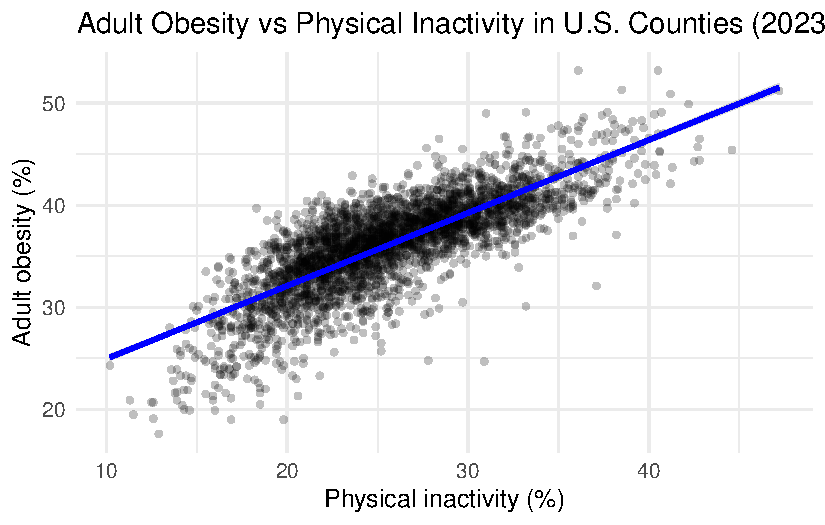
\includegraphics{paper_files/figure-pdf/fig-county-scatter-1.pdf}

}

\caption{\label{fig-county-scatter}Adult Obesity (\%) vs Physical
Inactivity (\%) --- U.S. Counties (2023). Points represent counties; the
solid line shows the OLS fit with a 95\% confidence band.}

\end{figure}%

\begin{ThreePartTable}
\begin{TableNotes}
\item \textit{Note: } 
\item Model fit: $R^{2}$ = 0.626, $R_{{adj}}^{2}$ = 0.626, Residual SE = 2.86, $n$ = 3191.
\item Because the sample size is large relative to the single predictor, the adjusted $R^{2}$ differs negligibly from the unadjusted value.
\end{TableNotes}

\begin{longtable}[t]{lrrrr}

\caption{\label{tbl-model}Regression of Adult Obesity (\%) on Physical
Inactivity (\%). Heteroskedasticity-consistent (HC1) standard errors
reported.}

\tabularnewline

\toprule
Term & Estimate & SE (HC1) & t-value & p-value\\
\midrule
Intercept & 17.811 & 0.299 & 59.59 & < 0.001\\
Inactivity (\%) & 0.714 & 0.011 & 64.77 & < 0.001\\
\bottomrule
\insertTableNotes

\end{longtable}

\end{ThreePartTable}

\subsection{Discussion}\label{discussion}

The fitted simple linear regression model provides a clear and
statistically robust summary of the association between physical
inactivity and adult obesity at the county level. The model explains
roughly ( 63\% ) of the total cross-county variation in obesity rates,
suggesting that inactivity alone is a major correlate of
population-level obesity.

Despite the high explanatory power and strong statistical significance (
( F = 5336,~p \textless{} 2 \times 10\^{}\{-16\} ) ), the model's
predictive precision for individual counties remains limited. The
residual standard error of ( 2.86 ) percentage points implies that
actual county obesity rates can deviate by approximately ( \pm 3 )
points from model-predicted values, even when inactivity levels are
known precisely. In addition, confidence intervals for mean predictions
are narrower than those for individual counties, reflecting the
uncertainty in predicting unobserved county outcomes.

The diagnostic analyses reveal a generally well-behaved model. Residuals
are centered and approximately homoscedastic, Q--Q plots show
near-normality with slight tail deviations, and no Cook's distance value
exceeds typical influence thresholds. These diagnostics confirm that OLS
assumptions are reasonably met, and the inference on the slope parameter
is statistically valid. Nevertheless, mild curvature in residual
patterns hints that the linear form could slightly understate the
association's complexity at extreme inactivity levels.

\subsection{Scope and Limitations}\label{scope-and-limitations}

The findings are \textbf{ecological}, reflecting county-level
associations rather than individual-level causal effects. The results
cannot be used to infer that physically inactive individuals are
necessarily obese; rather, counties with higher inactivity rates also
tend to have higher aggregate obesity rates. Several unmeasured
confounders---such as \textbf{age distribution, socioeconomic status,
built environment,} and \textbf{dietary patterns}---may jointly
influence both variables. Future research could extend this framework to
a \textbf{multiple regression model} incorporating these covariates to
test robustness and identify partial effects.

Moreover, the model is \textbf{cross-sectional}, describing associations
for a single year (2023). It does not capture temporal dynamics or
potential lag effects. Longitudinal modeling of panel data would provide
stronger evidence about persistence or causality in these relationships.

\section*{References}\label{references}
\addcontentsline{toc}{section}{References}

\phantomsection\label{refs}
\begin{CSLReferences}{1}{0}
\bibitem[\citeproctext]{ref-CHR2023}
County Health Rankings \& Roadmaps. 2023. {``County Health Rankings \&
Roadmaps: 2023 Ranked Measure Data.''}
\url{https://www.countyhealthrankings.org/}.

\bibitem[\citeproctext]{ref-R-base}
R Core Team. 2024. \emph{R: A Language and Environment for Statistical
Computing}. Vienna, Austria: R Foundation for Statistical Computing.
\url{https://www.r-project.org/}.

\bibitem[\citeproctext]{ref-broom}
Robinson, David, Alex Hayes, and Simon Couch. 2024. \emph{Broom: Convert
Statistical Objects into Tidy Tibbles}.
\url{https://broom.tidymodels.org/}.

\bibitem[\citeproctext]{ref-ggplot2-book}
Wickham, Hadley. 2016. \emph{Ggplot2: Elegant Graphics for Data
Analysis}. New York: Springer.

\bibitem[\citeproctext]{ref-ggplot2}
Wickham, Hadley, Winston Chang, Lionel Henry, Thomas Lin Pedersen,
Kohske Takahashi, Claus Wilke, Kara Woo, Hiroaki Yutani, Dewey
Dunnington, and PBC Posit Software. 2024. \emph{Ggplot2: Create Elegant
Data Visualisations Using the Grammar of Graphics}.
\url{https://ggplot2.tidyverse.org/}.

\bibitem[\citeproctext]{ref-dplyr}
Wickham, Hadley, Romain François, Lionel Henry, Kirill Müller, Davis
Vaughan, and PBC Posit Software. 2024. \emph{Dplyr: A Grammar of Data
Manipulation}. \url{https://dplyr.tidyverse.org/}.

\bibitem[\citeproctext]{ref-readr}
Wickham, Hadley, Jim Hester, and posit team. 2024. \emph{Readr: Read
Rectangular Text Data}. \url{https://readr.tidyverse.org/}.

\end{CSLReferences}




\end{document}
